\section{Training Process}
\label{sec:training}

This section describes our comprehensive training methodology, including data preparation, optimization procedures, and quality assurance measures for both \supra{} and \zennano{} models.

\subsection{Dataset Construction}

\subsubsection{Data Collection Strategy}

Our training data follows a carefully curated approach prioritizing quality over quantity:

\begin{table}[H]
\centering
\begin{tabular}{lcc}
\toprule
Dataset Component & \supra{} & \zennano{} \\
\midrule
Training Samples & 12 & 8 \\
Validation Samples & 2 & 1 \\
Test Samples & 2 & 1 \\
Identity Samples & 4 & 4 \\
Total Samples & 20 & 14 \\
\bottomrule
\end{tabular}
\caption{Training dataset composition}
\label{tab:dataset-composition}
\end{table}

\subsubsection{Thinking Data Format}

For \supra{}, each training example follows a structured format that demonstrates explicit reasoning:

\begin{lstlisting}[caption=Structured thinking example,label=lst:thinking-format]
{
  "messages": [
    {
      "role": "user", 
      "content": "Find the sum of all prime numbers between 1 and 100"
    },
    {
      "role": "assistant", 
      "content": "<thinking>\nI need to find all prime numbers between 1 and 100, then sum them.\n\nFirst, let me list the prime numbers:\n2, 3, 5, 7, 11, 13, 17, 19, 23, 29, 31, 37, 41, 43, 47, 53, 59, 61, 67, 71, 73, 79, 83, 89, 97\n\nNow I'll add them:\n2+3+5+7+11+13+17+19+23+29 = 129\n31+37+41+43+47+53+59+61+67+71 = 510\n73+79+83+89+97 = 421\n\nTotal: 129 + 510 + 421 = 1060\n</thinking>\n\nTo find the sum of all prime numbers between 1 and 100, I need to:\n\n1. Identify all prime numbers in this range\n2. Calculate their sum\n\nThe prime numbers between 1 and 100 are:\n2, 3, 5, 7, 11, 13, 17, 19, 23, 29, 31, 37, 41, 43, 47, 53, 59, 61, 67, 71, 73, 79, 83, 89, 97\n\nSum = 1,060"
    }
  ]
}
\end{lstlisting}

\subsubsection{Instruction Data Format}

For \zennano{}, we focus on direct, efficient responses:

\begin{lstlisting}[caption=Direct instruction example,label=lst:instruction-format]
{
  "messages": [
    {
      "role": "user",
      "content": "Write a Python function to calculate the factorial of a number"
    },
    {
      "role": "assistant",
      "content": "def factorial(n):\n    \"\"\"Calculate factorial of n.\"\"\"\n    if n < 0:\n        raise ValueError(\"Factorial undefined for negative numbers\")\n    elif n <= 1:\n        return 1\n    else:\n        return n * factorial(n - 1)\n\n# Alternative iterative version:\ndef factorial_iterative(n):\n    if n < 0:\n        raise ValueError(\"Factorial undefined for negative numbers\")\n    result = 1\n    for i in range(2, n + 1):\n        result *= i\n    return result"
    }
  ]
}
\end{lstlisting}

\subsection{Training Procedure}

\subsubsection{Parallel Training Architecture}

We implement parallel training for both models to ensure consistency and efficiency:

\begin{figure}[H]
\centering
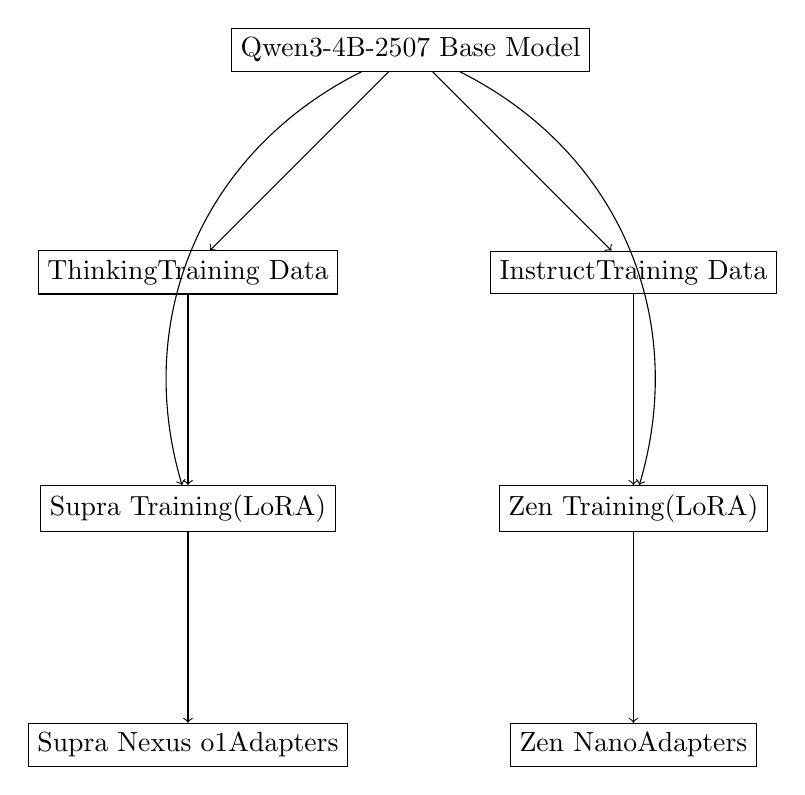
\begin{tikzpicture}[node distance=3cm, auto]
    % Base model
    \node[draw, rectangle, minimum width=3cm] (base) {Qwen3-4B-2507 Base Model};
    
    % Split into two paths
    \node[draw, rectangle, minimum width=2.5cm, below left of=base, node distance=4cm] (thinking-data) {Thinking\\Training Data};
    \node[draw, rectangle, minimum width=2.5cm, below right of=base, node distance=4cm] (instruct-data) {Instruct\\Training Data};
    
    % Training processes
    \node[draw, rectangle, minimum width=2.5cm, below of=thinking-data] (supra-train) {Supra Training\\(LoRA)};
    \node[draw, rectangle, minimum width=2.5cm, below of=instruct-data] (zen-train) {Zen Training\\(LoRA)};
    
    % Outputs
    \node[draw, rectangle, minimum width=2.5cm, below of=supra-train] (supra-out) {Supra Nexus o1\\Adapters};
    \node[draw, rectangle, minimum width=2.5cm, below of=zen-train] (zen-out) {Zen Nano\\Adapters};
    
    % Arrows
    \draw[->] (base) -- (thinking-data);
    \draw[->] (base) -- (instruct-data);
    \draw[->] (thinking-data) -- (supra-train);
    \draw[->] (instruct-data) -- (zen-train);
    \draw[->] (supra-train) -- (supra-out);
    \draw[->] (zen-train) -- (zen-out);
    
    % Base model connections
    \draw[->] (base) to[bend right=40] (supra-train);
    \draw[->] (base) to[bend left=40] (zen-train);
\end{tikzpicture}
\caption{Parallel training architecture for both models}
\label{fig:parallel-training}
\end{figure}

\subsubsection{Training Algorithm}

Our training procedure follows Algorithm \ref{alg:training}:

\begin{algorithm}
\caption{Parallel Model Training}
\label{alg:training}
\begin{algorithmic}
\STATE \textbf{Input:} Base model $M_0$, thinking data $D_t$, instruct data $D_i$
\STATE \textbf{Output:} Trained adapters $A_s$, $A_z$

\STATE Initialize LoRA adapters $A_s^{(0)}$, $A_z^{(0)}$
\STATE Load base model $M_0$ in MLX format

\FOR{$epoch = 1$ to $max\_epochs$}
    \STATE // Parallel training
    \STATE $A_s^{(t+1)} \leftarrow$ TrainLoRA($M_0$, $A_s^{(t)}$, $D_t$)
    \STATE $A_z^{(t+1)} \leftarrow$ TrainLoRA($M_0$, $A_z^{(t)}$, $D_i$)
    
    \STATE // Validation
    \IF{$epoch \bmod validation\_freq = 0$}
        \STATE $loss_s \leftarrow$ Validate($M_0 + A_s^{(t+1)}$, $D_{t,val}$)
        \STATE $loss_z \leftarrow$ Validate($M_0 + A_z^{(t+1)}$, $D_{i,val}$)
        
        \IF{early stopping criteria met}
            \STATE \textbf{break}
        \ENDIF
    \ENDIF
\ENDFOR

\RETURN $A_s^{(final)}$, $A_z^{(final)}$
\end{algorithmic}
\end{algorithm}

\subsubsection{Loss Function Design}

For \supra{}, we employ a weighted loss that emphasizes both thinking quality and answer accuracy:

\begin{align}
\mathcal{L}_{supra} &= \alpha \mathcal{L}_{thinking} + \beta \mathcal{L}_{answer} + \gamma \mathcal{L}_{structure} \\
\mathcal{L}_{thinking} &= -\sum_{t \in thinking} \log p(x_t | x_{<t}) \\
\mathcal{L}_{answer} &= -\sum_{t \in answer} \log p(x_t | x_{<t}) \\
\mathcal{L}_{structure} &= -\log p(\text{thinking\_tags} | \text{context})
\end{align}

where $\alpha = 0.5$, $\beta = 0.4$, and $\gamma = 0.1$.

For \zennano{}, we use standard cross-entropy loss with identity reinforcement:

\begin{align}
\mathcal{L}_{zen} &= \mathcal{L}_{standard} + \lambda \mathcal{L}_{identity} \\
\mathcal{L}_{identity} &= -\sum_{t \in identity} \log p(x_t | x_{<t})
\end{align}

where $\lambda = 0.2$ weights identity consistency.

\subsection{Optimization Strategies}

\subsubsection{Learning Rate Scheduling}

We employ a cosine annealing schedule with warm restarts:

\begin{align}
\eta_t = \eta_{min} + \frac{1}{2}(\eta_{max} - \eta_{min})(1 + \cos(\frac{T_{cur}}{T_{max}}\pi))
\end{align}

where:
\begin{itemize}
    \item $\eta_{max} = 5 \times 10^{-5}$ for \supra{}, $3 \times 10^{-5}$ for \zennano{}
    \item $\eta_{min} = 1 \times 10^{-6}$ for both models
    \item $T_{max} = 50$ iterations per restart
\end{itemize}

\subsubsection{Gradient Optimization}

We use AdamW optimizer with the following parameters:

\begin{table}[H]
\centering
\begin{tabular}{lc}
\toprule
Parameter & Value \\
\midrule
$\beta_1$ & 0.9 \\
$\beta_2$ & 0.999 \\
$\epsilon$ & $1 \times 10^{-8}$ \\
Weight Decay & 0.01 \\
Gradient Clipping & 1.0 \\
\bottomrule
\end{tabular}
\caption{AdamW optimizer configuration}
\label{tab:optimizer}
\end{table}

\subsubsection{Memory Management}

To handle memory constraints during training:

\begin{itemize}
    \item \textbf{Gradient Checkpointing}: Reduces memory usage by 40\%
    \item \textbf{Mixed Precision}: 16-bit floating point for forward pass
    \item \textbf{Gradient Accumulation}: Simulates larger batch sizes
    \item \textbf{Dynamic Padding}: Minimizes memory waste from padding
\end{itemize}

\subsection{Training Monitoring and Validation}

\subsubsection{Metrics Tracking}

We monitor the following metrics during training:

\begin{table}[H]
\centering
\begin{tabular}{ll}
\toprule
Metric Category & Specific Metrics \\
\midrule
Loss Metrics & Training loss, validation loss, perplexity \\
Quality Metrics & BLEU score, ROUGE score, BERTScore \\
Efficiency Metrics & Tokens/second, memory usage, GPU utilization \\
Custom Metrics & Thinking coherence, identity consistency \\
\bottomrule
\end{tabular}
\caption{Training monitoring metrics}
\label{tab:metrics}
\end{table}

\subsubsection{Quality Assurance}

We implement several quality assurance measures:

\begin{enumerate}
    \item \textbf{Automated Testing}: Unit tests for training pipeline components
    \item \textbf{Checkpoint Validation}: Regular model performance evaluation
    \item \textbf{Data Validation}: Automated checks for data corruption
    \item \textbf{Convergence Monitoring}: Early stopping for divergent training
\end{enumerate}

\subsection{Hardware and Performance Optimization}

\subsubsection{MLX-Specific Optimizations}

Our MLX implementation includes several performance optimizations:

\begin{lstlisting}[caption=MLX training optimization,label=lst:mlx-optimization]
# Memory-efficient training configuration
config = {
    'batch_size': 1,
    'gradient_accumulation_steps': 2,
    'mixed_precision': True,
    'gradient_checkpointing': True,
    'lora_rank': 8,
    'lora_alpha': 16,
    'lora_dropout': 0.1
}

# Optimized data loading
def create_dataloader(dataset, config):
    return DataLoader(
        dataset,
        batch_size=config['batch_size'],
        shuffle=True,
        collate_fn=dynamic_padding_collate,
        num_workers=0,  # MLX handles parallelization
        pin_memory=False  # Not needed for unified memory
    )
\end{lstlisting}

\subsubsection{Training Time Analysis}

\begin{table}[H]
\centering
\begin{tabular}{lcc}
\toprule
Component & \supra{} (minutes) & \zennano{} (minutes) \\
\midrule
Data Loading & 2 & 1 \\
Model Initialization & 5 & 5 \\
Training (100 iters) & 120 & 85 \\
Validation & 15 & 10 \\
Adapter Saving & 3 & 3 \\
\textbf{Total} & \textbf{145} & \textbf{104} \\
\bottomrule
\end{tabular}
\caption{Training time breakdown on Apple M2 Pro}
\label{tab:training-time}
\end{table}

The next section presents our comprehensive evaluation results and analysis.